\begin{figure}[t!]
\begin{subfigure}{.8\columnwidth}
  \centering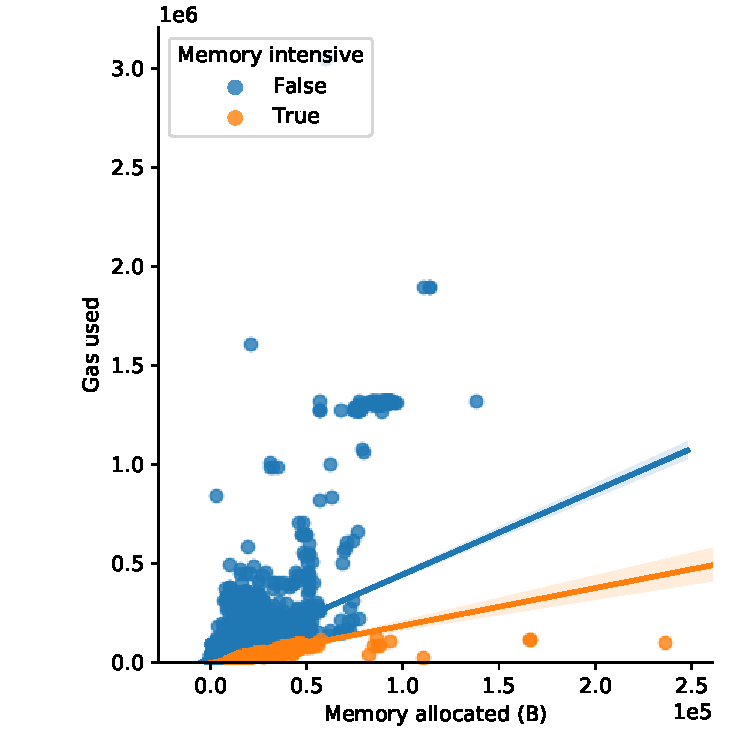
\includegraphics[width=.8\columnwidth]{figures/memory-usage-1400000-1500000.pdf}
  \caption{Pre EIP~150 correlation between gas and memory usage.}
  \label{fig:gas-memory-pre-eip150}
\end{subfigure}

\begin{subfigure}{.8\columnwidth}
  \centering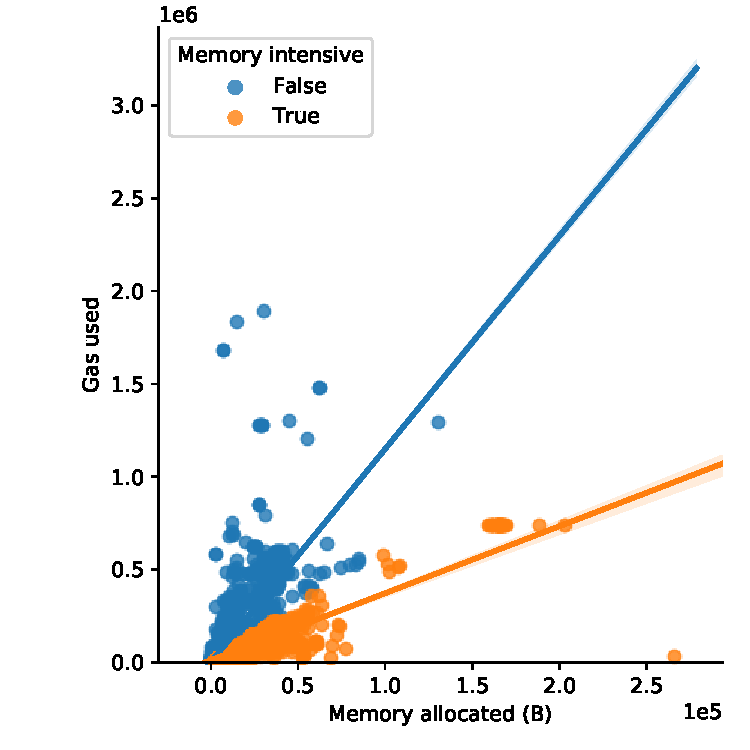
\includegraphics[width=.8\columnwidth]{figures/memory-usage-2500000-2600000.pdf}
  \caption{Post EIP~150 correlation between gas and memory usage.}
  \label{fig:gas-memory-post-eip150}
\end{subfigure}

\begin{subfigure}{.9\columnwidth}
  \centering
  \begin{tabular}{clrr}
    \toprule
    \thead[l]{Phase} & \thead[l]{Executions\\set} & \thead[r]{Pearson\\score} & \thead[r]{Gas/byte}\\
    \midrule
    \multirow{3}{*}{Pre EIP~150} & $E$ & 0.545 & 3.96\\
    & $E_{MI}$ & 0.773 & 1.80\\
    & $E \setminus E_{MI}$ & 0.633 & 4.96\\
    \midrule
    \multirow{3}{*}{Post EIP~150} & $E$ & 0.755 & 7.67\\
    & $E_{MI}$ & 0.902 & 4.16\\
    & $E \setminus E_{MI}$ & 0.907 & 11.7\\
    \bottomrule
  \end{tabular}
  \caption{Relation between allocated memory and gas usage.}
  \label{tab:gas-memory-relation}
\end{subfigure}
\caption{Correlation between gas and memory usage.}
\end{figure}

\section{Analysis of Gas Consumption}
\label{sec:analysis}

In this section, we analyse the gas consumption of Ethereum smart contracts and try to correlate it with different system resources, such as memory, CPU and storage.
To measure the consumption, we re-execute the Ethereum blockchain with a patched version of the Ethereum C++ client~\cite{aleth} and collect information about resources for each contract invocation. As described in Section~\ref{sec:background}, EIP~150 influenced the price of many storage related operations, which affected the gas cost of transactions. Therefore, we perform our experiments on a set of ~\empirical{100,000} blocks before EIP~150 and a set of~\empirical{100,000} blocks after EIP~150. EIP~150 was introduced at height~\empirical{2,463,000}. We arbitrarily use block~\empirical{1,400,000} to block ~\empirical{1,500,000} for measurements before EIP~150 and block ~\empirical{2,500,000} to~\empirical{2,600,000} for measurements after EIP~150. Although the block numbers are arbitrary, we assume that the sample of~\empirical{100,000} blocks which roughly corresponds to two weeks, is large enough to obtain reliable data.

Below, we denote the gas usage for a transaction as $G$. All the figures in this section include bands marking a confidence interval of 95\%.

\subsection{Memory Usage}
 We note $M_{+}$ the amount of memory allocated and $M_{-}$ the amount of memory deallocated. We compute the extra amount of memory allocated $M = M_{+} - M_{-}$ to execute a particular transaction, that is, the difference between the total amount of memory allocated and the total amount of memory deallocated.

An important point is that contracts which allocate storage in any way, may it be with \lstinline{SSTORE} instructions or \lstinline{LOG} instructions, will see their memory overhead increase, as this extra storage will stay in memory even after the execution of the contract. Although this is not a perfect measurement, as part of the memory may be released later on during the execution of the transaction, it does give a proxy measure of how a particular contract execution affects the memory usage of the client. It is also worth noting that some contracts may also release more memory than they allocate, if, for example, a contract self-destructs itself. As we want to focus on how execution can consume resources, we filter contracts where~$M < 0$.

We first compute the Pearson correlation coefficient\footnote{Pearson score of 1 means perfect positive correlation, 0 means no correlation}~\cite{boslaugh2012statistics} between the extra memory allocated and the gas usage. For contracts prior to  EIP~150, we obtain a score \empirical{0.545} which shows that, although a positive correlation exists between memory and gas usage, the correlation is fairly weak. As described in Section~\ref{sec:background}, EIP~150 influenced widely the price of all storage related operations, which vastly affect the results obtained for memory usage. Indeed, the Pearson correlation coefficient we obtain for post EIP~150 data is~\empirical{0.766}. This shows that the correlation between memory and gas usage is vastly greater after EIP~150.

The data we obtain suggest that there are different trends in terms of correlation between gas and memory usage. Therefore, we decide to separate the data in two categories to try to isolate the two trends. We first compute the ratio of extra memory allocated per gas used: $R_{M/G} = M / G$. The higher the ratio is, the lower a transaction is paying to consume memory. We then split in~10 quantiles and assign the quantile with the highest ratio $R_{M/G}$, that is, the quantile paying the less gas for memory, as being ``Memory intensive''. We define $E$ the set of all executions and $E_{MI}$ as the set of ``memory intensive'' executions.

We plot our results pre and post EIP~150 in Figure~\ref{fig:gas-memory-pre-eip150} and in Figure~\ref{fig:gas-memory-post-eip150}. We also show the correlation scores we obtain as well as the relation between gas usage and memory usage in Figure~\ref{tab:gas-memory-relation}. The gas/byte column represents the cost in gas to allocate one extra byte of memory and is inferred by performing a linear regression on the data.

There are several interesting points to note about the results. First, EIP~150 resulted in a significant increase in the price of gas per memory, which had the effect of increasing the correlation between these two variables. Second, after EIP~150, the difference between normal and memory intensive contracts becomes more visible, with the gas per byte cost going from~\empirical{4.16} for memory intensive contract executions up to~\empirical{11.7} for others. Nevertheless, both type of contracts have a high correlation score between gas and memory allocated. This shows that there are important discrepancies on how pricing is done for consumed memory depending on the characteristics of the contract being executed.

\begin{figure}[tb]
  \centering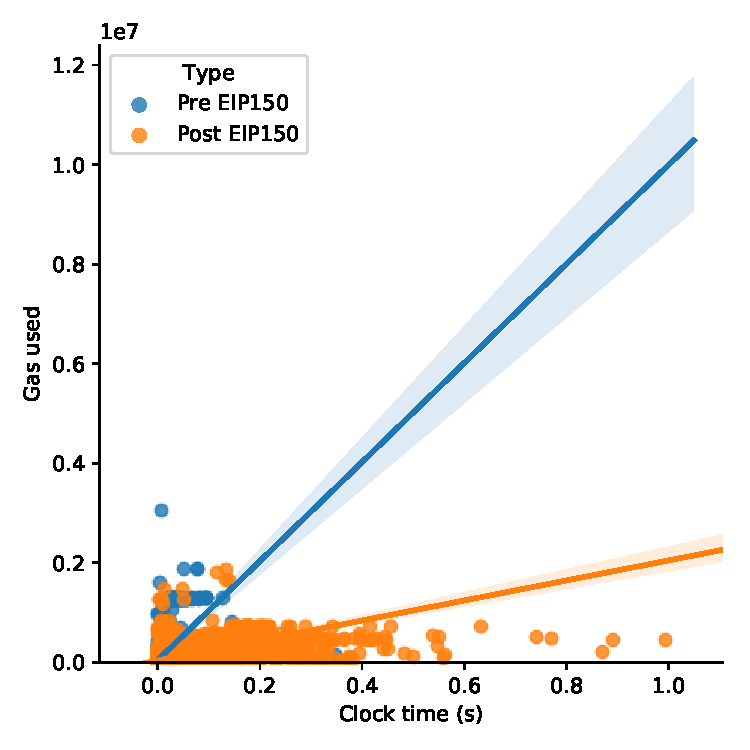
\includegraphics[width=.8\columnwidth]{figures/cpu-usage-1400000-1500000--2500000-2600000.pdf}
  \caption{Correlation between gas and CPU usage.}
  \label{fig:gas-cpu}
\end{figure}

\subsection{CPU Usage}
We analyse the correlation between the gas usage and the CPU usage for each transaction. As for the memory measurements, we use our instrumented C++ client and record the number of clock ticks used by the thread executing the transaction. We use this clock time as a proxy for the CPU usage.

Again, we compute the Pearson correlation score between the CPU and gas usage. The score for contract executions before EIP~150 is~\empirical{0.528} while the score after EIP~150 is~\empirical{0.507}. This score implies a low positive correlation between the two variables. This comes from the fact that the instructions touching to storage are very expensive, thus dominating the cost of other instructions. The score most likely got lower after EIP~150 because storage related operations got more expensive.

We plot the relation between the CPU and gas usage before and after EIP~150 in Figure~\ref{fig:gas-cpu}. Although the correlation is fairly low, it is interesting to see that with EIP~150, as a consequence of storage related operation increasing, the relative cost of CPU has decreased.

\begin{figure}[tb] \centering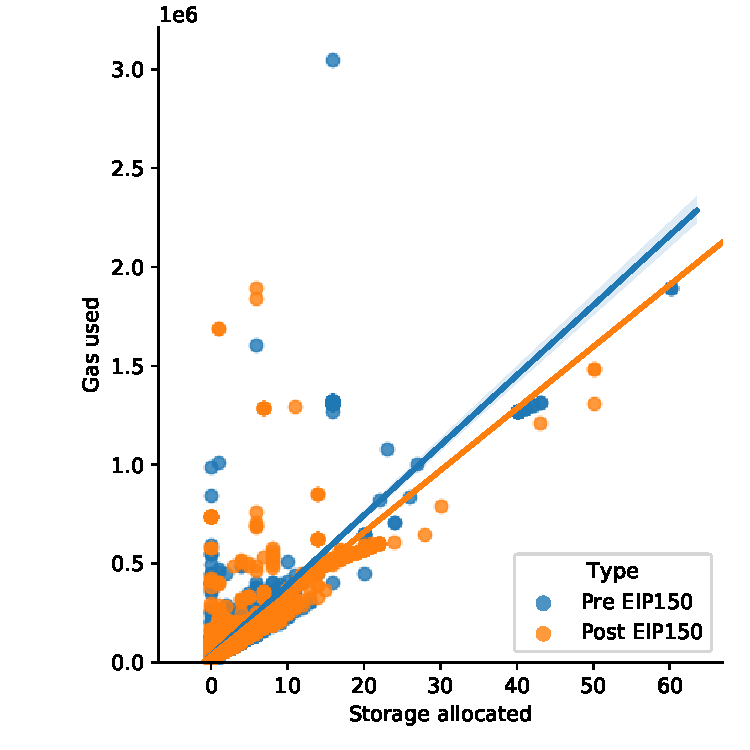
\includegraphics[width=.8\columnwidth]{figures/storage-usage-1400000-1500000--2500000-2600000.pdf}
  \caption{Correlation between gas and storage usage.}
  \label{fig:gas-storage}
\end{figure}

\subsection{Storage Usage}
To analyse the storage usage, we analyse the number of EVM words~(256 bits) of storage allocated per transactions. Here, we define a word to have been allocated if its value before a transaction was 0 and its value after the transaction was not. Conversely, a word has been deallocated if its value before a transaction was non-zero and its value after is~0. Both of these costs are formally defined in Ethereum~\cite{wood2014ethereum} and the main goal of this experiment is to see by how much the storage allocation dominates the total gas cost. The number of allocations made during a single execution can be negative, if more words are deallocated than allocated. Again, as we focus on the resource usage, we filter out this type of executions.

We compute the Pearson's correlation before and after EIP~150 and obtain respectively~\empirical{0.821} and~\empirical{0.907}. This shows that there is, as expected, a strong positive correlation between the amount of storage allocated and the gas cost during a single execution.
We plot the relation between the storage allocated and the gas used before and after EIP~150 in Figure~\ref{fig:gas-storage}. Although EIP~150 increased the price for a lot of storage related instructions, it changed neither the price of allocating a new value, nor the reimbursement received when deallocating a value. This explains that, unlike for memory, the cost does not go up after EIP~150. An interesting point to notice is that the execution cost does not split into two different gas usage trends as they do with memory, which suggests that the storage cost is not what is creating this effect for the extra memory allocated.

\begin{figure}[tb]
  \centering
  \setlength{\tabcolsep}{10pt}  
  \begin{tabular}{clr}
    \toprule
    \thead[l]{Phase} & \thead[l]{Resources} & \thead[r]{Pearson\\score}\\
    \midrule
    \multirow{4}{*}{Pre EIP~150} & Memory/CPU & 0.591\\
    & Storage/CPU & 0.725\\
    & Storage/Memory & 0.845\\
    & Storage/Memory/CPU & 0.759\\
    \midrule
    \multirow{4}{*}{Post EIP~150} & Memory/CPU & 0.741\\
    & Storage/CPU & 0.837\\
    & Storage/Memory & 0.938\\
    & Storage/Memory/CPU & 0.893\\
    \bottomrule
  \end{tabular}
  \caption{Multivariate correlation between gas and resources.}
  \label{tab:multivar-correlation-scores}
\end{figure}

\subsection{Multi-variate Correlation}
Instead of simply using a bi-variate correlation between gas consumption and a resource, we try to correlate gas consumption to multiple resources at a time. To compute the multi-variate correlation between multiple resources and the gas usage, we proceed as follow.

Given $n$ measures for $m$ resources $r_1, \cdots, r_m$, we note $R_1, \cdots, R_m$ the vectors of measures for each resource, which will each have a dimension of $n$. We first use equation~\ref{eq:normalize} to normalise each vector $R_i$ to a new vector $R'_i$ so that each vector $R'_i$ has a mean of 0 and a standard deviation of 1. We note $\overline{R_i}$ the mean of $R_i$ and $\sigma_{R_i}$ its standard deviation.

\begin{equation}
  \label{eq:normalize}
  R'_i = \frac{R_{i} - \overline{R_i}}{\sigma_{R_i}}
\end{equation}
%
We then concatenate vectors $R'_1,\cdots,R'_m$ into a $n\times m$ matrix $M$ and use a principal component analysis~\cite{abdi2010principal} to reduce the dimension of $M$ to $n\times 1$. The vector we obtain represent the aggregated usage of the different resources. We finally compute the Pearson's correlation score between this vector and the gas used. We show the results we obtain in Figure~\ref{tab:multivar-correlation-scores}.

Overall we find that for both pre- and post-EIP~150 measurements the aggregation of memory and storage correlates best with gas usage. On the opposite, the CPU usage seem to be adding more noise than information and adding the CPU usage always result in a lower correlation than without it.

\begin{figure}[tb]
  \centering
  \setlength{\tabcolsep}{14pt}
  \begin{tabular}{clr}
    \toprule
    \thead[l]{Phase} & \thead[l]{Resource} & \thead[r]{Pearson\\score}\\
    \midrule
    \multirow{4}{*}{Pre EIP~150} & Memory & 0.773\\
    & CPU & 0.528\\
    & Storage & 0.775\\
    & Storage/Memory & 0.845\\
    \midrule
    \multirow{4}{*}{Post EIP~150} & Memory & 0.755\\
    & CPU & 0.507\\
    & Storage & 0.907\\
    & Storage/Memory & 0.938\\
    \bottomrule
  \end{tabular}
  \caption{Correlation between gas and resources.}
  \label{tab:correlation-scores}
\end{figure}

\subsection{Summary}
Overall, we have seen that the gas usage is dominated by the \emph{storage allocated}, which can also be approximated reasonably well by the memory allocation during a single contract execution. On the other hand, given the high cost of storage, we find that CPU usage and gas usage correlate poorly. 
We summarise all bi-variate correlations as well as the best performing multivariate correlation in Figure~\ref{tab:correlation-scores}.
